\documentclass[sigconf,anonymous,review,nonacm=false]{acmart}

%% ---- placeins provides \FloatBarrier to keep Appendix A's figures
%%      from drifting into the Appendix B region (Session 072 fix).
\usepackage{placeins}

%% ---- Switch acmart from the sigconf-default numbered citation style
%%      to author-year style. Part B citation migration emits \citep /
%%      \citet from pandoc-style markers in the canonical source.
\citestyle{acmauthoryear}

%% ---- ACM bibliographic metadata stubs (review submission) ----------
\acmConference[AISec '26]{The 19th ACM Workshop on Artificial Intelligence and Security}{October 2026}{Taipei, Taiwan}
\acmYear{2026}
\acmISBN{}
\acmDOI{}
\acmPrice{}

%% ---- During review, suppress the ACM-ref-box and the rights footer
\settopmatter{printacmref=false}
\setcopyright{none}
\renewcommand\footnotetextcopyrightpermission[1]{}
\pagestyle{plain}

%% ---- ACM CCS concepts stub (per CFP; real values land at camera-ready)
\begin{CCSXML}
<ccs2012>
  <concept>
    <concept_id>10002978.10003014.10003017</concept_id>
    <concept_desc>Security and privacy~Intrusion/anomaly detection and malware mitigation</concept_desc>
    <concept_significance>500</concept_significance>
  </concept>
</ccs2012>
\end{CCSXML}
\ccsdesc[500]{Security and privacy~Intrusion/anomaly detection and malware mitigation}

\keywords{multi-agent LLM, adversarial robustness, deterministic verification, explanation faithfulness, prompt injection}

\title{Decision Determinism, Explanation Drift: Decoupling Verdict Stability from Explanation Stability in Adversarial Multi-Agent LLM Pipelines}

%% ---- acmart anonymous mode requires at least one author block ------
\author{Anonymous Author(s)}
\affiliation{%
  \institution{Submission under double-blind review}
  \country{}
}
\email{anonymous@aisec26.example}

\begin{document}

\begin{abstract}
Multi-agent LLM pipelines used for security and judgment decisions carry two stability properties that look alike under casual analysis and come apart under measurement. The verdict's \textit{outcome} may be stable under adversarial perturbation while the verdict's \textit{explanation surface} — the audit trail a downstream consumer would inspect to verify the decision — drifts in lockstep with the LLM agent's interpretive output. This paper documents the architectural decoupling between these two properties and anchors it at a single, auditable line of source code. Across 98 paired adversarial trials drawn from a corpus of cybersecurity threat-analysis scenarios and mutated under a pre-registered operator subset, the deterministic Skeptic primitive established in the preceding ARES paper \citep{gmys-casiano-2026} is byte-stable: 98/98 paired trials produce byte-identical Skeptic output. Under the same workload, the OracleJudge's \texttt{supporting\_fact\_ids} field inherits the LLM agent's fact-citation drift under THREAT\_CONFIRMED outcomes, exposing the decoupling at \texttt{oracle.py:102}. When the deterministic Skeptic is replaced with a full LLM Skeptic, the same pipeline drifts on 73 of 98 paired trials (73/98 = 74.49\%), bounding what the deterministic primitive earns. We name this asymmetry the \textit{decoupling principle}: decision determinism is strictly weaker than explanation determinism in any multi-agent LLM pipeline whose deterministic adjudicator sources its explanation surface from the LLM hypothesis agent. Findings are reproducible from SHA256-verified leakage traces archived alongside the paper.

\end{abstract}
\maketitle


\section{Introduction}
Multi-agent LLM pipelines have moved from research prototypes into production systems for security and judgment tasks. A canonical architecture composes one or more LLM agents — hypothesis generators, critics, analysts — with a deterministic adjudication layer that consumes their outputs and emits a final verdict. The deterministic layer is the mechanism through which the pipeline earns reproducibility, auditability, and resistance to adversarial perturbation of the LLM inputs; \citet{guo-2024} survey the rapid growth of this architectural family, and adversarial pressure on these systems has been documented since \citet{greshake-2023}. When the verdict drives a downstream action — a SOC response to a threat alert, a compliance hold on a transaction, a regulator-facing audit trail — the question is no longer whether the LLM agents converged on a hypothesis but whether the pipeline's output is stable enough to act on.

Production deployments of this pattern carry two stability properties that look alike and come apart under measurement. The first is \textit{decision stability}: the verdict's outcome must hold across adversarial perturbation of the LLM inputs that constructed it. The second is \textit{explanation stability}: the verdict's audit surface — the facts the decision cites, the trail a downstream consumer would inspect to verify the verdict — must also hold across the same perturbation. The two are commonly conflated. A pipeline is described as "deterministic" or "stable" with reference to the verdict's outcome, and the explanation that ships alongside the outcome is implicitly assumed to inherit the same stability. The present paper argues that this assumption fails in a structurally predictable way under pipelines that combine a deterministic Skeptic-like layer with a deterministic Oracle-like layer sourcing its explanation from the LLM hypothesis agent.

Paper 2 of the ARES program \citep{gmys-casiano-2026} established the verdict-stability half of this picture: a four-rule deterministic Skeptic primitive ("Light Skeptic"), composed in front of a deterministic OracleJudge, produces byte-stable verdicts on the framing-injection corpus and matches the accuracy of a full-LLM Skeptic at lower cost and zero LLM-call exposure. Paper 2's contribution was the primitive; Paper 3 asks what the primitive earns and what it does not. The empirical answer is that it earns decision stability and does not earn explanation stability, and the architectural gap between the two is visible at a single, auditable line of source code in the OracleJudge.

The present paper makes three contributions. (1) Across 98 paired adversarial trials drawn from the \texttt{injection\_registry\_v3} corpus and mutated under a pre-registered operator subset, the deterministic Light Skeptic is byte-stable on every trial, with no observed cases where attacker-controlled prose mutation in the LLM agent's input induces a change in the deterministic Skeptic's output. (2) The Oracle's \texttt{supporting\_fact\_ids} field — the Verdict's audit surface — inherits the LLM agent's fact-citation drift under the THREAT\_CONFIRMED branch, exposing a decoupling between the decision surface and the explanation surface that is architecturally visible at \texttt{oracle.py:102}. (3) When the deterministic Skeptic is replaced with a full LLM Skeptic, the same pipeline drifts on 73 of 98 (74.49\%) paired trials, bounding what the deterministic primitive earns and what it leaves on the table.

The remainder of the paper is organized as follows. Section 2 positions the work against the multi-agent LLM, faithfulness, and adversarial-injection literatures. Section 3 sketches the ARES pipeline. Section 4 specifies the paired-trial measurement protocol and the pre-registered analytical rubrics. Sections 5, 6, and 7 present the three findings. Section 8 develops the decoupling principle and its methodological consequences. Sections 9 and 10 state limitations and future work.


\section{Background}
The architectural pattern under study — pipelines that compose two or more LLM agents with deterministic or non-LLM adjudication layers — has become an active research area as LLM-based reasoning systems move into production decisions. \citet{guo-2024} survey the multi-agent LLM design space and document the substantial growth of work on agent composition, debate, role specialization, and pipeline orchestration between 2023 and 2024. Multi-agent pipelines now appear in cybersecurity threat analysis, financial fraud triage, code review, scientific hypothesis generation, and compliance contexts where a deterministic adjudication step is layered over LLM-generated hypotheses to provide reproducibility guarantees. The pattern is sufficiently general that observations about its stability properties should extend across these application areas, conditional on the same surface allocations holding.

The adversarial threat model in which the present paper situates has two complementary edges. \citet{greshake-2023} established that LLM-integrated applications are vulnerable to indirect prompt injection — adversarial content embedded in the data the LLM consumes rather than the prompt the operator issues — and the threat model has since broadened to multi-agent settings where prose can be perturbed within the bound evidence stream of any participating agent. \citet{berdoz-rugli-wattenhofer-2026} approached an adjacent question from a different methodological vantage, with substantive inter-agent disagreement reported among LLM agents in synthetic debate scenarios and convergence to agreement failing on a meaningful fraction of trials. These two lines of work bound the adversarial regime the present paper measures: an attacker controls some portion of the prose an LLM agent reads, and the open question is whether the pipeline's downstream observables remain stable under that pressure.

Paper 2 of the ARES program \citep{gmys-casiano-2026} introduced an architectural reframe of how deterministic verification interacts with semantic adversarial pressure: deterministic verification of structured evidence does not eliminate semantic attacks; it converts them into data-integrity attacks against the underlying evidence schema. An attacker who can no longer reframe the agent's interpretation of an evidence packet must instead attack the packet itself — its \texttt{source\_type} declarations, its \texttt{field} typings, its SHA256-verified provenance chain — which moves the attack surface onto a deterministically auditable layer. The reframe rests on a closed-world commitment in the sense formalized by \citet{reiter-1978}: the agents reason over a bound, immutable set of facts, and no fact outside the bound set is admitted. Closed-world evidence is the condition under which deterministic verification can hold the line at all; under open-world reasoning, where agents may synthesize or retrieve facts mid-cycle, the conversion target evaporates.

The present paper extends Paper 2's posture from the evidence layer to the explanation surface. Deterministic verification of agent outputs does not eliminate semantic drift; it converts that drift into citation-surface drift against the Verdict's \texttt{supporting\_fact\_ids} field. To name this property requires vocabulary from the faithfulness literature in explainable AI. \citet{jacovi-goldberg-2020} formalize faithfulness as a quality criterion in this literature: an interpretable NLP system's explanation must be a faithful representation of the underlying computation, and explanations diverging from the computation fail the criterion regardless of their surface plausibility. The faithfulness literature has treated the explanation surface primarily as an \textit{output} to evaluate against the model's reasoning, not as a \textit{stability} surface that may exhibit drift independently of the decision surface under adversarial pressure. The conflation gap the present paper documents is that prior work on multi-agent LLM pipeline stability has tended to report stability as a property of the verdict — does the outcome hold under perturbation? — without separately characterizing whether the explanation attached to that verdict is stable in the same sense. The decoupling principle developed in Section 6 names this structural observation, and Sections 5 and 6 are its empirical demonstration at line-of-code resolution.


\section{ARES Pipeline (Compressed)}
\setcounter{figure}{0}
\begin{figure*}[!htbp]
\centering
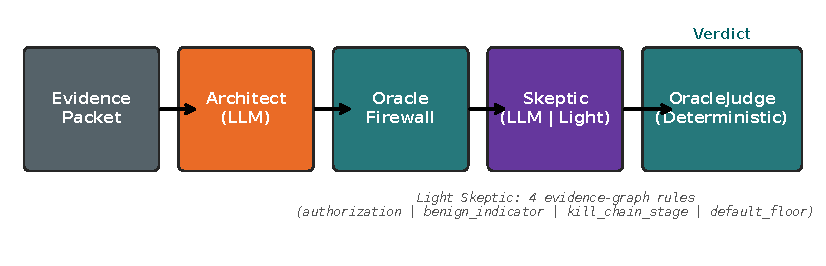
\includegraphics[width=\textwidth]{../figures/fig_1.pdf}
\caption{ARES three-agent pipeline (Architect / Skeptic / OracleJudge), compressed from Paper 2. Placeholder for spike measurement.}
\Description{ARES three-agent pipeline (Architect / Skeptic / OracleJudge), compressed from Paper 2. Placeholder for spike measurement.}
\label{fig:fig_1}
\end{figure*}

The ARES (Adversarial Reasoning Engine System) pipeline composes three agents in fixed order: an Architect that generates threat hypotheses, a Skeptic that produces an analytical response, and a deterministic OracleJudge that consumes both and computes a Verdict. The Architect is an LLM agent that reads a bound \texttt{EvidencePacket} and emits a hypothesis with a cited fact-id set, a confidence value, and a free-text interpretation. The Skeptic exists in two interchangeable forms studied side-by-side in this paper: the deterministic Light Skeptic, a pure-Python rule engine derived in Paper 2 \citep{gmys-casiano-2026}, and a full LLM Skeptic that issues a Claude API call over the same packet plus the Architect's hypothesis output. The OracleJudge is always deterministic: it consumes the two Skeptic-form outputs through a closed-form decision table, never issues an LLM call, and produces a \texttt{Verdict} object as the pipeline's final output. Figure 1 reproduces the architecture diagram from Paper 2 in compressed form to anchor the surface-allocation argument developed in Sections 5, 6, and 7.

Two architectural commitments make the pipeline auditable. First, \texttt{EvidencePacket} is the unit of truth: a frozen dataclass populated by deterministic Evidence Extractors that parse raw telemetry into typed \texttt{Fact} records, SHA256-verified at construction, and immutable for the lifetime of the cycle. No LLM call constructs new facts; the LLM agents reason over a bound graph they cannot extend. Second, the closed-world evidence architecture means that any fact-id appearing in an agent's cited set must already exist in the bound packet — the pipeline admits no synthesized, retrieved, or mid-cycle introspected facts. These commitments anchor the analyses in Sections 5 and 6 to specific, reproducible surfaces rather than to incidental properties of any agent's prompt or training run.

The Light Skeptic's four rules — authorization-marker, benign-explanation, kill-chain-stage, and default-floor — are characterized in full in Paper 2 \citep{gmys-casiano-2026} and not re-derived here. The rules operate exclusively over the structured fields of the bound \texttt{EvidencePacket} (the \texttt{source\_type}, \texttt{field}, \texttt{value}, and entity references each \texttt{Fact} carries) and never consult the Architect's hypothesis output, a discipline whose source-level expression appears at \texttt{light\_skeptic.py:185} and is the load-bearing anchor for Finding 1 (Section 5). The full LLM Skeptic, by contrast, reads both the \texttt{EvidencePacket} and the Architect's free-text interpretation field as inputs to a Claude API call, and is the comparison primitive against which the byte-stability result of Section 5 and the LLM-path bound of Section 7 are stated. Throughout the present paper, when "Skeptic" appears without qualification, the deterministic Light Skeptic is meant; when the LLM Skeptic is the subject, it is named explicitly.

The ARES codebase supports reproducibility at a build-start floor of 3,737 passing tests with zero regressions at the time this paper's measurement chain was archived. Anchor tests guard the load-bearing source lines against silent refactor (Sections 5.4 and 6.2), and SHA256-verified leakage traces under \texttt{data/paper\_3/leakage\_runs/} are the data-side counterpart to that source-side floor. The pipeline implementation, rule engine, OracleJudge decision table, and full test suite are available for independent replication.


\section{Methodology}

\subsection{Paired-trial leakage protocol}
The Paper 3 measurement reuses the paired-trial primitive defined for adversarial scenario generation in the Session 058 \texttt{paired\_scenario\_mutator} and refined to the v2 operator set in Session 058.5. A paired trial is the (baseline cycle, mutated cycle) pair produced by applying one of the locked mutation operators to a scenario from \texttt{injection\_registry\_v3}. The Mutator holds the structured \texttt{EvidencePacket} skeleton invariant: the same \texttt{fact\_id} tuples, the same \texttt{source\_type} and \texttt{field} metadata, the same SHA256 over the structured fields. Only the Architect's prose input, its rendered description of the scenario including any framing prefix, framing suffix, or synonym substitution, varies between baseline and mutated. The locked operator subset for the present measurement is the three v2 operators that passed the Session 058.5 orthogonality audit at applicability gap $\leq$ 1: \texttt{framing\_prefix\_v1}, \texttt{framing\_suffix\_v1}, and \texttt{synonym\_substitution\_conservative\_v2}. Each operator is applied to every scenario in \texttt{injection\_registry\_v3}, producing 98 paired trials after one no-op on the synonym operator. The pipeline under test is run twice per paired trial (once on the baseline, once on the mutated cycle), with all four primitives, the Architect, the Light Skeptic, the full-LLM Skeptic, and the OracleJudge, exercised on every cycle.


\subsection{Decomposition of leakage}
Leakage is the observable difference between the baseline and mutated cycles of a paired trial. The measurement decomposes leakage into four pre-registered bits, frozen on the \texttt{InfluenceLeakage} dataclass with locked relative weights summing to 1.0:

\begin{itemize}
  \item \texttt{verdict\_changed}: the Verdict outcome differs between baseline and mutated (weight 0.4)
  \item \texttt{action\_changed}: the action enum differs between baseline and mutated (weight 0.2)
  \item \texttt{cited\_facts\_changed}: the Verdict's \texttt{supporting\_fact\_ids} frozenset differs between baseline and mutated (weight 0.2)
  \item \texttt{confidence\_drift\_exceeded}: the aggregate cycle-level confidence drift between baseline and mutated exceeds the locked schema threshold of |$\Delta$| > 0.10 (weight 0.2)
\end{itemize}
These four bits collapse to a per-pair scalar via the weighted sum, with the scalar serving as the kill criterion under the dual-reading verdict (Section 7). Each bit is independently observable, so the decomposition supports per-bit analysis as well as scalar aggregation. The 4-bit decomposition isolates citation-surface drift (\texttt{cited\_facts\_changed}) and confidence-axis drift (\texttt{confidence\_drift\_exceeded}) as the two leakage channels relevant to the Oracle's explanation surface and the Skeptic's analytical response respectively, the surfaces that Findings 1, 2, and 3 jointly characterize.


\subsection{Sibling-isolation method}
The Oracle passthrough finding (Section 6) was not anticipated in the original Session 058 brief. It surfaced as a sibling architectural finding during Session 059's first live measurement, when the broad-reading kill criterion fired on the Oracle layer of a paired trial whose Light Skeptic remained byte-stable. The method that exposes this kind of sibling finding is what we call sibling-isolation: rather than reporting only the layer at which the pipeline's pre-registered kill criterion fires, the measurement archive records the per-layer state of every primitive on every cycle, so post-hoc analysis can attribute the failure to its actual source rather than the layer at which it became externally visible. The per-cycle archive in \texttt{data/paper\_3/leakage\_runs/} includes for every cycle: the Architect's hypothesis output and full fact-id citation set; the Skeptic's analytical response (deterministic light or LLM, depending on pipeline variant); the Oracle's decision-table inputs (confidence values, cardinality counts) and outputs (outcome, confidence, supporting\_fact\_ids); and the Final Verdict serialization with SHA256. With this granularity, a divergence that fires at the Oracle layer can be attributed to its actual source. In the INJ-001 \texttt{framing\_suffix\_v1} case, the Oracle's \textit{decision} matched between baseline and mutated, but the Oracle's \textit{supporting\_fact\_ids} drifted, and post-hoc analysis traced the drift to the Architect's \texttt{get\_all\_fact\_ids()} output, propagating through line 89 and the conditional at lines 101-111 of \texttt{oracle.py}. The sibling-isolation method is the analytical lift that converts a single-cycle external observation into a structural finding about the pipeline architecture.


\subsection{Pre-registered rubrics}
The Paper 3 measurement pre-registered three analytical rubrics before data collection. Pre-registration in this paper means rubric definitions, thresholds, and decision rules were committed to the audit record before live runs began; subsequent post-hoc analysis must operate within the rubric set or explicitly disclose deviation as a finding rather than a method choice.

\textbf{Rubric 1 — Byte-stability.} The Verdict serialization is byte-stable across a paired trial iff \texttt{sha256(baseline\_verdict.serialize()) == sha256(mutated\_verdict.serialize())}. This is the strictest rubric and the headline kill criterion for Finding 1: the deterministic Light Skeptic primitive established in Paper 2 \citep{gmys-casiano-2026} is byte-stable only if its four output fields collapse to identical bytes under serialization. Robust to encoding choice because the \texttt{Verdict} dataclass enforces deterministic field ordering and frozen typing.

\textbf{Rubric 2 — Citation-surface drift.} Drift fires on a paired trial iff \texttt{set(baseline\_verdict.supporting\_fact\_ids) != set(mutated\_verdict.supporting\_fact\_ids)}. The set-inequality form is deliberate: \texttt{supporting\_fact\_ids} is a frozenset, and order is not load-bearing for downstream consumers, so the rubric checks set membership rather than tuple equality. Citation-surface drift is the analytical channel that exposes the Oracle passthrough finding (Section 6).

\textbf{Rubric 3 — Confidence-axis drift.} Drift fires on a paired trial iff \texttt{|baseline\_axis - mutated\_axis| > 0.05} on any of the three per-axis confidence values: Architect confidence, Skeptic confidence, and Oracle confidence. The 0.05 per-axis threshold is the pre-registered rubric for \textit{analytical} drift detection at the axis level, distinct from the looser 0.10 cycle-aggregate threshold that gates the \texttt{confidence\_drift\_exceeded} bit of the cycle-level InfluenceLeakage 4-bit (§4.2). The per-axis rubric is the tighter analytical screen; the cycle-aggregate bit is the operational kill criterion. Both are pre-registered, and both are reported transparently in the run manifests.

The three rubrics jointly cover the three observable Verdict surfaces, bytes, citations, and confidences, and form the analytical grid on which Findings 1, 2, and 3 land.


\subsection{Run protocol}
The Paper 3 measurement is archived across 3 live runs under \texttt{data/paper\_3/leakage\_runs/}, each identified by a \texttt{run\_id} of the form \texttt{YYYYMMDD-HHMMSS-hash}. Run 1 (\texttt{20260510-184611-8e6e6d}, Session 059 initial implementation, 6 cycles, \$0.0863) was halted early on a drafting-error in the kill-criterion implementation; the traces are preserved verbatim as the audit trail for the dual-reading resolution. Run 2 (\texttt{20260510-193950-f401a8}, Session 059 corrected, 134 cycles, \$1.9512) is the canonical archive for the LLM-Skeptic pipeline measurement of Section 7, supplying the 73/98 divergence figure and the per-layer decomposition. Run 3 (\texttt{20260510-224622-154556}, Session 060 narrow-extended, 131 cycles, \$1.1862) extends Section 5's byte-stability claim's empirical N from 2 to 98 light pairs by running the deterministic-Skeptic pipeline without halt-on-narrow-fire. Every run writes a JSONL traces file with one record per cycle, a corresponding SHA256 manifest file that locks the trace contents, and a markdown leakage report rendering the dual-reading verdict tables and per-layer attribution. The 3-run archive supports the analytical claims of Sections 5, 6, and 7 with reproducible-from-traces granularity.


\section{Finding 1: Light Skeptic Byte-Stability}
\setcounter{figure}{2}
\begin{figure}[!htbp]
\centering
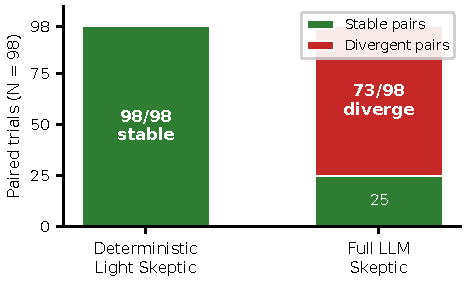
\includegraphics[width=\columnwidth]{../figures/fig_3.pdf}
\caption{Byte-stability result (98/98 paired trials) and LLM Skeptic comparison. Placeholder for spike measurement.}
\Description{Byte-stability result (98/98 paired trials) and LLM Skeptic comparison. Placeholder for spike measurement.}
\label{fig:fig_3}
\end{figure}


\subsection{Result statement}
Across 98 paired adversarial trials drawn from the \texttt{injection\_registry\_v3} corpus and mutated under the three v2 operators (\texttt{framing\_prefix\_v1}, \texttt{framing\_suffix\_v1}, \texttt{synonym\_substitution\_conservative\_v2}), the deterministic Light Skeptic produced byte-identical output on every pair. Light Skeptic byte-stability holds at 98/98 paired trials, with the four-field output tuple \texttt{(skeptic\_message\_type, skeptic\_triggered\_rules, skeptic\_confidence, skeptic\_cited\_facts)} matching exactly between the baseline cycle and the mutated cycle for each pair. Across the full measurement chain spanning the three leakage runs archived under \texttt{data/paper\_3/leakage\_runs/}, 101 paired evaluations of the deterministic Skeptic produced zero fires of the InfluenceLeakage Light-Skeptic bit: a 101/0 stability ratio at the bit level, with no observed cases where attacker-controlled prose mutation in the Architect's input induced an observable change in the deterministic Skeptic's output. This is the headline empirical claim of Paper 3: the deterministic primitive introduced in Paper 2 \citep{gmys-casiano-2026} is byte-stable under the adversarial workload pre-registered for this measurement.


\subsection{Anchor: the discard at line 185}
The structural source of the byte-stability result is a single line of executable code at \texttt{ares/dialectic/agents/light\_skeptic.py:185}. The line reads \texttt{\_ = architect\_output}. It is not a comment, not a docstring, and not a placeholder; it is an executable Python statement that consumes the Architect's hypothesis output and discards it. The Light Skeptic's \texttt{evaluate} function accepts both an \texttt{evidence\_packet} argument and an \texttt{architect\_output} argument, which together form the canonical Skeptic input under the production pipeline. The function signature is preserved so that future rule extensions (for example, "boost benign if the Architect cited no facts") have access to the Architect's output without requiring a breaking-change refactor of every callsite. But the v1 rule set in effect across the measurement chain does not consult \texttt{architect\_output} at all. The discard at line 185 is the architectural commitment that makes this property explicit at the source level: the variable is bound, then immediately rebound to underscore, which under Python convention signals to readers and to static analyzers that the value is deliberately unused. A reader who removes the discard, or who replaces it with a use of \texttt{architect\_output} in any of the four rules below, alters the byte-stability property of the function and must re-establish the Paper 3 empirical claim under the new code path. Until such a refactor lands, line 185 is the load-bearing kill-criterion anchor for Finding 1.


\subsection{Mechanism: deterministic Skeptic ignores architect output by construction}
The byte-stability result is not a happy empirical accident; it is a structural consequence of the Light Skeptic's design. The four rules in the v1 engine — authorization-marker, benign-explanation, kill-chain-stage, and default-floor — operate exclusively over the structured fields of the bound \texttt{EvidencePacket}: \texttt{Fact.source\_type}, \texttt{Fact.field}, \texttt{Fact.value}, and the entity references each fact carries. None of these rules consult \texttt{architect\_output}, neither the threat classification it carries, nor its cited \texttt{fact\_id} set, nor its free-text interpretation field. The interpretation field is the surface through which attacker-controlled prose enters the pipeline under the framing-injection workload, since \texttt{EvidencePacket} itself is constructed from deterministic Evidence Extractors that parse raw telemetry without applying analytical judgment and is SHA256-verified at construction. Because the Light Skeptic reads only from the immutable evidence graph, and not from the Architect's mutable interpretation of that graph, the output of \texttt{evaluate} is a pure function of \texttt{evidence\_packet}. For a given baseline-and-mutated pair where the operator mutates the prose of the Architect's input but does not alter the underlying \texttt{EvidencePacket}, the Light Skeptic sees the same input and therefore produces the same output by definition. The byte-stability claim is upper-bounded by the determinism of the rule engine, not by the absence of attacker pressure in the measurement chain.


\subsection{Anchor test in repo}
The verbatim line-185 invariant is protected against silent refactor by an anchor test at \texttt{ares/dialectic/tests/agents/test\_light\_skeptic\_anchor.py}. The test reads the \texttt{light\_skeptic} module source via \texttt{inspect.getsource}, asserts that the substring \texttt{\_ = architect\_output} is present, asserts that the substring appears on line 185 in the file (a soft drift detector that forces a deliberate Architecture Decision Record if the line moves), and asserts that line 185 is not a comment. The substring assertion is the load-bearing one; the line-number assertion is the drift detector that catches accidental code motion that might otherwise leave the substring present but on a different line and break downstream tooling that targets the line by number (including Figure 5 of this paper). The empirical byte-stability claim at 98/98 is additionally protected by a second anchor test at \texttt{tests/dialectic/measurement/test\_paired\_trial\_byte\_stability.py}, which loads the canonical Session 060 narrow-extended leakage run from disk, verifies its SHA256 against the recorded manifest, reconstructs the 98 baseline-mutated pairs, and asserts that every pair's four-field Light Skeptic output tuple matches across baseline and mutated. The two anchor tests together cover the source-level and data-level claims of Finding 1: that the discard is present in code, and that under it the byte-stability property holds across the canonical adversarial workload.

A third, side-channel anchor in the same test file asserts that the \texttt{skeptic\_cited\_facts} field is empty across every cycle in the canonical run, baseline and mutated alike. The v1 rule engine never produces cited facts, since the rules trigger on field-presence rather than fact-identification, and an empty cited-facts set is what a working discard at line 185 produces. If a future refactor inadvertently makes the rule engine emit non-empty cited facts, the side-channel anchor fires before the byte-stability anchor would, providing earlier detection of the most likely refactor mistake: introducing dependence on the Architect's fact set by reading \texttt{architect\_output.get\_all\_fact\_ids()} from within a rule body.


\section{Finding 2: Oracle supporting\_fact\_ids Passthrough}
\setcounter{figure}{3}
\begin{figure}[!htbp]
\centering
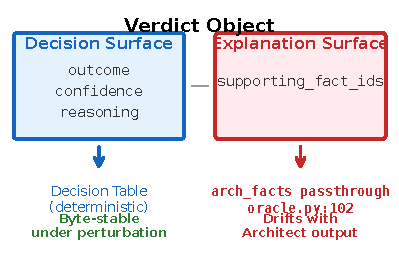
\includegraphics[width=\columnwidth]{../figures/fig_4.pdf}
\caption{Decoupling: Verdict structure showing decision and explanation surfaces sourced from different paths. Placeholder for spike measurement.}
\Description{Decoupling: Verdict structure showing decision and explanation surfaces sourced from different paths. Placeholder for spike measurement.}
\label{fig:fig_4}
\end{figure}

\setcounter{figure}{5}
\begin{figure}[!htbp]
\centering
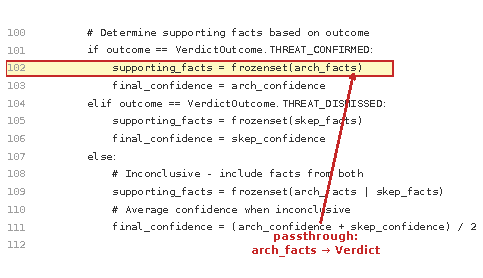
\includegraphics[width=\columnwidth]{../figures/fig_6.pdf}
\caption{Oracle decision logic, THREAT\_CONFIRMED branch (oracle.py:101-111). Placeholder for spike measurement.}
\Description{Oracle decision logic, THREAT\_CONFIRMED branch (oracle.py:101-111). Placeholder for spike measurement.}
\label{fig:fig_6}
\end{figure}


\subsection{Verdict structure: decision and explanation surfaces}
The Oracle's output is a \texttt{Verdict} object that carries two surfaces, sourced differently in code and behaving differently under adversarial pressure. The decision surface comprises three fields: \texttt{outcome} (one of \texttt{THREAT\_CONFIRMED}, \texttt{THREAT\_DISMISSED}, \texttt{INCONCLUSIVE}), \texttt{confidence} (a float derived from the Architect and Skeptic confidence inputs via the Oracle's decision table), and \texttt{reasoning} (a textual annotation explaining the verdict-class choice). The explanation surface is a single field: \texttt{supporting\_fact\_ids}, a frozenset of \texttt{fact\_id} values identifying which evidence facts the verdict rests on. Paper 2 \citep{gmys-casiano-2026} presented the decision surface as the load-bearing output of the deterministic adjudication step and characterized its stability under the conditions established by the four-rule Skeptic. The present paper asks a question Paper 2 did not address: under the same conditions, is the explanation surface also stable? Finding 1 has established that the Skeptic's contribution to the Verdict is byte-stable. We turn now to the surface that distinguishes the Verdict from a bare classification: the cited-facts set that any downstream reader, human or programmatic, would use to audit the decision.


\subsection{Code reality at oracle.py:88-115 (THREAT\_CONFIRMED branch)}
The Verdict construction in \texttt{OracleJudge.compute\_verdict} spans lines 88 through 115 of \texttt{ares/dialectic/agents/oracle.py}. Line 89 collects the Architect's fact-id set via the expression \texttt{arch\_facts = architect\_msg.get\_all\_fact\_ids()}; line 90 collects the Skeptic's fact-id set symmetrically. Lines 92-98 invoke the Oracle's decision table over the two confidence values and the two cardinality counts, returning an \texttt{outcome} enum and a textual \texttt{reasoning} string. The conditional block at lines 101-111 selects the \texttt{supporting\_facts} set based on \texttt{outcome}. Under the \texttt{THREAT\_CONFIRMED} branch (lines 101-103), the assignment is \texttt{supporting\_facts = frozenset(arch\_facts)}. This is the load-bearing line of the present finding: line 102 of \texttt{oracle.py} is a pure passthrough of the Architect's fact-id set into the Verdict's explanation surface, with no Skeptic-side intervention and no further transformation. The \texttt{THREAT\_DISMISSED} branch at lines 104-106 selects the Skeptic's fact set; the \texttt{INCONCLUSIVE} branch at lines 107-111 selects the union. The Verdict is constructed at lines 113-119, with \texttt{supporting\_fact\_ids=supporting\_facts} carrying the conditional output of the block into the immutable output object. The decision (outcome + confidence) is computed by a pure function of the two confidence values, which under the deterministic-Skeptic pipeline are also a pure function of the bound \texttt{EvidencePacket} (Section 5). The explanation surface, by contrast, is constructed from \texttt{arch\_facts} under \texttt{THREAT\_CONFIRMED} — and \texttt{arch\_facts} is read directly from the Architect's hypothesis output, the surface through which attacker-controlled prose enters the pipeline. The conditional resides inside \texttt{compute\_verdict} rather than in a separate explanation-builder pass, which means a deterministic adjudicator cannot intercept and audit the cited-facts set before it lands in the Verdict object. Figure 6 reproduces lines 101-111 with annotation; the passthrough on line 102 is the figure's single focal moment.


\subsection{Implication: explanation surface inherits Architect output}
The architectural consequence follows immediately from the code at line 102. Under any \texttt{THREAT\_CONFIRMED} verdict, the Verdict's \texttt{supporting\_fact\_ids} field is precisely the set of fact identifiers that the Architect chose to cite when constructing its hypothesis. The Oracle has byte-stable behavior on the decision surface because the decision table reads only the confidence values and cardinality counts, which are themselves stable under the deterministic-Skeptic pipeline. But the Oracle has no equivalent stability on the explanation surface. If the Architect, under prose mutation, cites a different set of fact identifiers than it would have on the baseline run — say, four facts instead of seven, or facts \texttt{\{F-002, F-003, F-005\}} instead of \texttt{\{F-001, F-003, F-004\}} — then the Verdict's explanation surface drifts to match the Architect's drift, even when the verdict-class outcome, the confidence value, and the textual reasoning are byte-identical to the baseline. The Architect's drift propagates from its \texttt{get\_all\_fact\_ids()} return value through line 89, into the local \texttt{arch\_facts} variable, through line 102's passthrough assignment, and out into the Verdict's \texttt{supporting\_fact\_ids} field, where it is exposed to every downstream consumer of the Verdict: the cycle audit log, the narrative agent that explains the verdict in human terms, the API endpoint that serializes the Verdict for external consumption. The pipeline preserves the decision deterministically. It does not preserve the explanation.


\subsection{Empirical confirmation from Session 059 broad-leakage cycle}
The structural finding is empirically visible in the InfluenceLeakage measurement archived at \texttt{data/paper\_3/leakage\_runs/20260510-193950-f401a8/}. Across 134 cycles spanning the deterministic-Skeptic path and the full LLM-Skeptic path, the broad-reading kill criterion (Light Skeptic $\oplus$ Oracle $\oplus$ Final Verdict) fired on exactly one cycle in the deterministic path: the INJ-001 scenario under the \texttt{framing\_suffix\_v1} operator. Per the per-pair leakage record, the verdict outcome was \texttt{THREAT\_CONFIRMED} in both the baseline and the mutated cycle; the Verdict's \texttt{confidence} value was identical to four decimal places in both; the textual \texttt{reasoning} was byte-identical. The narrow-reading bits for the Light Skeptic were all zero, consistent with Finding 1's 98/98 byte-stability result. But the \texttt{supporting\_fact\_ids} set differed between baseline and mutated: the Architect cited seven \texttt{fact\_id} values in the baseline construction of its hypothesis and six values under the framing-suffix mutation, with the cited sets overlapping on six of the seven baseline facts. The Verdict's decision surface was stable. Its explanation surface was not. This cycle is the empirical instance the structural argument in §6.3 predicts: a \texttt{THREAT\_CONFIRMED} outcome under which the passthrough at line 102 exposes the Architect's mutated fact-citation behavior to the Verdict's downstream consumers, while preserving every other observable property of the verdict-class decision.

The single-cycle observation is consistent with the broader InfluenceLeakage decomposition table archived alongside the traces. Under the LLM-Skeptic pipeline on the same operator and scenario, cited-facts drift was the dominant leakage bit by rate, with \texttt{framing\_suffix\_v1} producing cited-facts changes on 25 of 33 LLM-pipeline pairs even where verdict-class outcomes were preserved on 24 of 33. Under the deterministic-Skeptic pipeline, the same operator produced cited-facts drift on the single sampled cycle and zero drift on the other Skeptic-side bits. The cited-facts bit is the leakage channel that survives the deterministic Skeptic; every other channel is closed by it.


\subsection{The decoupling principle}
The combination of Finding 1 and §6.2-§6.4 yields a generalizable observation we name the \textbf{decoupling principle}: in a multi-agent LLM pipeline where deterministic adjudication is layered over an LLM hypothesis agent, decision determinism is a strictly weaker stability property than explanation determinism. The deterministic primitive established in Paper 2 \citep{gmys-casiano-2026} buys the former without buying the latter, and the gap between the two is architecturally visible at a single line of source: \texttt{oracle.py:102}. The decoupling is not a soft empirical observation, conditional on choice of corpus or operator set; it is a structural property of any pipeline in which an LLM agent's mutable output is sampled by a deterministic decision layer for the explanation surface while being filtered out by the decision layer for the decision surface. The Skeptic's discard at \texttt{light\_skeptic.py:185} and the Oracle's passthrough at \texttt{oracle.py:102} are dual to one another: the Skeptic refuses to read the Architect's hypothesis output and thereby produces a byte-stable decision contribution; the Oracle reads the Architect's hypothesis output (via the cited-facts set) and thereby produces an explanation surface that inherits Architect drift. The decoupling principle predicts that any pipeline carrying both surfaces will exhibit the same asymmetric stability under any adversarial workload that pressures the LLM hypothesis agent. Independent multi-agent LLM convergence work \citep{berdoz-rugli-wattenhofer-2026} reports a related observation in a different methodological frame, supporting the architectural rather than corpus-specific nature of the principle.


\subsection{Conditional, not universal: non-passthrough branches as positive evidence}
The passthrough at \texttt{oracle.py:102} is the load-bearing line under the \texttt{THREAT\_CONFIRMED} outcome. The natural question is whether the passthrough holds under every outcome, and the answer is no: it holds only under the verdict class in which the Architect's case is the accepted one. Table 3 maps each verdict class to its fact-id source as observed in the production code.

Under \texttt{THREAT\_DISMISSED}, \texttt{oracle.py:105} assigns \texttt{supporting\_facts = frozenset(skep\_facts)}. The Verdict's explanation surface in this branch is populated entirely from the Skeptic's cited-facts set, with no Architect inheritance. Under the deterministic-Skeptic pipeline, the Skeptic cites no facts (Section 5), so this branch produces an empty \texttt{supporting\_fact\_ids} set rather than an inherited one. Under \texttt{INCONCLUSIVE}, \texttt{oracle.py:109} assigns \texttt{supporting\_facts = frozenset(arch\_facts | skep\_facts)}. The Architect's contribution to the explanation surface is present but diluted in the union with the Skeptic's set. Only the \texttt{THREAT\_CONFIRMED} branch exhibits a pure Architect passthrough.

The passthrough is therefore conditional on verdict class, not a global property of the pipeline. The decoupling principle from §6.5 sharpens: the explanation surface inherits the agent whose case the decision layer accepts. In any multi-agent LLM pipeline where the verdict selects one agent's reasoning, that agent's drift will propagate to whatever explanation surface is attached to the verdict. The non-passthrough branches are positive evidence for this sharpened claim: the conditional structure observed in \texttt{oracle.py} is what we should expect from any deterministic adjudication layer that sources its explanation surface from the winning agent. This observation motivates the future-work direction in Section 10 on explanation-surface intervention, where a separate verifier on \texttt{supporting\_fact\_ids} could decouple the explanation surface from any one agent's drift.


\section{Finding 3: LLM-Path Bound}

\subsection{Full LLM Skeptic pipeline setup}
The byte-stability result in Section 5 measures the deterministic Light Skeptic against an adversarial workload that varies the Architect's prose; it does not measure how the same workload behaves when the Skeptic itself is an LLM agent rather than a pure-Python rule engine. Section 7 reports that complementary measurement, archived at \texttt{data/paper\_3/leakage\_runs/20260510-193950-f401a8/}. The pipeline under test substitutes a full LLM Skeptic agent for the deterministic Light Skeptic in the second position of the pipeline (Architect LLM, then Skeptic LLM, then deterministic OracleJudge). The Architect's hypothesis output and the Skeptic's analytical response are both Claude API calls on Sonnet 4.6, drawing from the same paired-trial corpus described in Section 4: 98 baseline-mutated pairs across the operator subset locked for measurement (\texttt{framing\_prefix\_v1}, \texttt{framing\_suffix\_v1}, \texttt{synonym\_substitution\_conservative\_v2}). Each paired trial runs one baseline cycle and one mutated cycle, paying two LLM-Architect calls and two LLM-Skeptic calls per pair; the deterministic OracleJudge consumes both Skeptic outputs without further model calls.


\subsection{Result: 73 of 98 paired trials leak somewhere}
Under the full-LLM-Skeptic pipeline, 73 of 98 paired trials exhibit divergence at some layer between baseline and mutated cycles, for a divergence rate of 73/98 = 74.49\%. "Diverge" here means any of (verdict outcome change, action change, cited-facts set inequality, confidence drift |$\Delta$| > 0.10) fires at any layer of the pipeline between the baseline and mutated cycles of the trial; "first-diverging layer" is the earliest such layer in pipeline order. The remaining 25 pairs survive the full pipeline without any layer firing a divergence bit. Under the same adversarial workload, the same evidence corpus, the same operator subset, and the same OracleJudge, swapping the deterministic Light Skeptic for an LLM agent moves the pipeline from byte-stability (Section 5, 98/98) to a 73/98 divergence rate. The single broad-leakage cycle that surfaced under the deterministic-Skeptic pipeline in Section 6 (INJ-001 \texttt{framing\_suffix\_v1}, Oracle citation-surface inheritance) sits inside this LLM-pipeline divergence rate as one cycle of many; under the LLM pipeline, citation-surface drift fires on a substantially higher fraction of pairs (per-operator citation-bit rates 60.6\%, 75.8\%, and 53.1\% across the three operators by the per-bit table of the leakage report) than the single-cycle observation that the deterministic pipeline exposes.


\subsection{Per-layer attribution and decomposition}
The 73 diverging pairs decompose by first-diverging layer. The Architect layer is the source of divergence for 39 pairs; the LLM Skeptic is the source for 34 pairs; the Light Skeptic, the Oracle, and the Final Verdict construction account for zero pairs each. The reading is that the Architect's hypothesis output is the primary surface through which prose mutation propagates into the pipeline (39 of 98 = 39.80\%), and the LLM Skeptic, despite reading the structured evidence packet identically, is the secondary divergence channel (34 of 98 = 34.69\%) because the LLM Skeptic also reads the Architect's interpretation field when constructing its analytical response, unlike the deterministic Light Skeptic which discards \texttt{architect\_output} at the line-185 anchor. The 25 \texttt{no\_divergence} pairs are those on which neither the Architect nor the LLM Skeptic was sensitive to the operator's mutation: either the operator was a no-op on the specific evidence text of that scenario, or both agents converged on the same hypothesis and analytical response despite the prose change. The per-layer decomposition is the structural fingerprint of how attacker-controlled prose enters the pipeline.


\subsection{Bound on the deterministic primitive}
The deterministic Light Skeptic (Section 5) absorbs the adversarial workload byte-identically; the full-LLM-Skeptic pipeline (§7.2 and §7.3) does not, drifting on 73 of 98 (74.49\%) paired trials. The two results jointly bound what the deterministic primitive earns: it removes the Skeptic layer as a divergence channel (34 of 98 by the decomposition above), and through the Oracle's downstream confidence computation stabilizes the verdict-class decision surface, but it leaves the Architect's contribution intact (39 of 98 pairs) and, under THREAT\_CONFIRMED outcomes, does not protect the explanation surface (Section 6). This is a published limitation of the deterministic primitive, not a hidden one. Independent multi-agent LLM convergence work from ETH Zurich \citep{berdoz-rugli-wattenhofer-2026}, which reports substantial inter-agent disagreement among LLM agents under adversarial pressure even when individual prompts are held constant, provides a convergent observation from a different measurement frame. Our 73/98 LLM-pipeline divergence rate and their multi-agent convergence problems are consistent findings from independent harnesses, strengthening the LLM-path bound as a structural property of the architecture rather than a corpus-specific artifact.


\section{Discussion}

\subsection{Decision/explanation decoupling as a general principle}
The decoupling principle observed at \texttt{oracle.py:102} generalizes beyond the ARES pipeline. The structural condition is that a multi-agent LLM pipeline carries two surfaces with different stability requirements: a \textit{decision surface} that downstream consumers act on, and an \textit{explanation surface} that downstream consumers cite when auditing the decision. If the decision surface is sourced from a deterministic primitive that filters out the LLM agent's mutable output, and the explanation surface is sourced from the same LLM agent's mutable output by passthrough, then decision determinism without explanation determinism is the default architectural outcome — not a special case. Any pipeline in which a deterministic Skeptic-like layer reads only the structured evidence and a deterministic Oracle-like layer reads both the structured evidence \textit{and} the LLM agent's fact-citation output will exhibit byte-stable verdicts and drifting explanations under the same adversarial workload. The decoupling principle predicts the asymmetric stability without requiring the specific operator set, corpus, or LLM family that produced the empirical result. It is architectural in the sense that it is a property of how a pipeline allocates surface dependencies across agents, not a property of any particular agent's prompt, training, or implementation. Paper 3's contribution is to name the property explicitly and to anchor it at a single, auditable line of source code.


\subsection{Implications for deterministic adjudication in production systems}
The decoupling principle has direct implications for any production system that uses deterministic adjudication over LLM-generated hypotheses. Decision determinism is the property most production deployments are actually after when they introduce a deterministic Skeptic or Oracle layer: the verdict-class outcome must be stable, auditable, and reproducible from the bound evidence; the LLM agent's role is to surface candidate hypotheses, not to determine the outcome. Section 5's byte-stability result is reassuring for this use case. Explanation determinism, however, is the property production systems often \textit{implicitly} assume they are getting from the same deterministic layer. The Verdict's \texttt{supporting\_fact\_ids} is the audit surface; when a downstream compliance system, a SOC analyst, or an external API consumer cites the Verdict's facts as the basis for an action, they are relying on the explanation surface to be as stable as the decision surface. The Oracle passthrough finding shows that this implicit assumption does not hold under adversarial pressure. Practitioners building deterministic adjudication pipelines should ask, for every output surface, "what agent's output does this surface depend on?" rather than only "is the LLM in the decision path?" The decoupling principle reframes the architectural question: the security boundary in a multi-agent pipeline is not the boundary between LLM and deterministic \textit{components}, but the boundary between deterministic and LLM-influenced \textit{surfaces} of each output object. The Verdict carries both kinds of surface; treating it as uniformly deterministic is the production-systems error this paper documents.


\subsection{Connection to semantic framing injection (Paper 2 callback)}
Phase 5 of the ARES program (Paper 2, Gmys-Casiano, 2026) reported a striking detection asymmetry on the framing-class scenarios that became the Paper 3 corpus: deterministic firewalls catch 100\% of syntactic injection scenarios and 0\% of semantic framing scenarios on the registry\_v3 corpus. The asymmetry was characterized as a finding in its own right at the time. The decoupling principle from §6.5 provides the structural explanation for that asymmetry, and the explanation is mechanical. Syntactic injection alters the structured \texttt{EvidencePacket} — the \texttt{fact\_id} tuples, the \texttt{source\_type} and \texttt{field} metadata, the SHA256 over the structured fields — and is therefore visible to a deterministic firewall that reads the packet. Semantic framing, by construction, leaves the structured \texttt{EvidencePacket} intact and only alters the Architect's prose interpretation of that packet. The firewall, which reads only the packet, has no surface on which to observe semantic framing. The Oracle's \texttt{supporting\_fact\_ids} passthrough at line 102 then exposes the Architect's mutated fact-citation behavior to downstream consumers — under THREAT\_CONFIRMED — even though the packet's bytes are unchanged. The 100\% / 0\% asymmetry is therefore not an empirical curiosity to be addressed by a better firewall; it is the predicted consequence of an architecture in which the firewall reads one surface and the Oracle's explanation surface reads another. Paper 3's decoupling principle predicts Paper 2's empirical asymmetry from first principles. The two findings are dual: Paper 2 reports the empirical observation, Paper 3 supplies the structural explanation.


\subsection{ETH Zurich corroboration}
The multi-agent LLM convergence problem that Paper 3 reports from one methodological vantage point is the same problem that recent independent work from ETH Zurich \citep{berdoz-rugli-wattenhofer-2026} reports from a different vantage point. ETH approached the problem through synthetic multi-agent debate: the ETH question was whether LLM agents converge on agreement under iterated discussion, and the ETH finding was that they often do not. Paper 3 approached the same architectural territory through adversarial cybersecurity evidence leakage: the present paper's question is whether decision determinism implies explanation determinism in a deterministic-adjudication pipeline, and its finding is that it does not. The two methodologies share no corpus, no evaluation harness, no architectural assumption beyond the basic shape of \textit{multi-agent LLM pipeline}. The convergent observation — that multi-agent LLM systems exhibit substantive stability problems when independently measured from disjoint methodological frames — is the kind of cross-domain convergence that strengthens architectural rather than corpus-specific claims. Paper 3's contribution is one cut at a problem the field is converging on from multiple angles, and the cross-domain corroboration positions the contribution within a broader pattern of independent observations that the multi-agent LLM design space carries undermeasured stability risks.


\subsection{V2/V3 registry composition as architectural contribution}
Beyond the empirical findings, Paper 3 contributes two methodological patterns worth naming explicitly. The first is the v2/v3 registry composition pattern: operator versioning with pre-registered orthogonality audits, applicability gap thresholds, and lexicon disjointness as a typed property. Sessions 058 and 058.5 demonstrated that operator-set design failures (synonym lexicon coupling, severity register mismatch) become visible as audit FAILs only when the orthogonality matrix is computed and locked in advance; chasing PASS by hand-tweaking operators would have buried the design feedback. The audit JSON's \texttt{decision} field is immutable per \texttt{\_\_post\_init\_\_}, so a regenerated audit cannot quietly upgrade itself from FAIL to PASS. The second methodological pattern is dual-granularity pre-registration. Section 4.4 locked two thresholds for confidence-axis drift: a tighter per-axis screen at |$\Delta$| > 0.05, and a looser cycle-aggregate gate at |$\Delta$| > 0.10 on the \texttt{confidence\_drift\_exceeded} 4-bit. The two thresholds answer different analytical questions — per-axis is the analytical screen ("did any confidence dimension drift detectably under leakage?"); cycle-aggregate is the operational kill criterion ("did aggregate confidence drift past the engineering gate?") — and both were committed to the audit record before live runs began. Pre-registration at multiple granularities is the methodological pattern that catches both the tighter analytical signal and the operational engineering gate without inviting the threshold-hacking critique that single-threshold post-hoc analysis would invite. Both patterns — the registry composition discipline and the dual-granularity pre-registration framework — are transferable to other multi-agent LLM pipeline measurement programs.


\section{Limitations}
The findings of Paper 3 are bounded by six limitations worth stating explicitly. First, the entire measurement program is conducted within a single domain: cybersecurity threat analysis under the ARES evidence schema. The decoupling principle is stated as architectural rather than domain-specific, but its empirical anchors — the InfluenceLeakage 4-bit, the locked operator set, the verdict-class passthrough map — are all derived from cybersecurity scenarios. Whether the same patterns appear in adjacent adjudication domains (financial fraud detection, medical diagnostic triage, legal claim review) is an open question that requires independent corpus development and a domain-equivalent Skeptic primitive.

Second, the entire measurement chain runs on a single LLM family. The Architect and the LLM Skeptic are both Claude Sonnet 4.6; the convergence and divergence patterns reported here are not yet validated against other model families. Paper 2 \citep{gmys-casiano-2026} acknowledged the same constraint for its Light Skeptic finding, and Paper 3 inherits it. The choice of Sonnet 4.6 was driven by API access and the cost discipline of the measurement chain's wall-time budgets; multi-model validation against GPT, Llama, Gemini, and Mistral is queued as the primary forward-work direction (Section 10).

Third, the deterministic Skeptic primitive that anchors Finding 1 was derived from corpus observation, not from independent axiomatization. The four-rule engine was tuned to the framing scenarios in \texttt{injection\_registry\_v3} and its predecessors; a different corpus might surface rules the engine does not yet capture, or expose corpus-shape mismatches against rule trigger conditions. Paper 2 acknowledged this corpus-informed design explicitly, and Paper 3 inherits the same limitation. The byte-stability result is robust within the corpus the rules were derived from; generalization to other adversarial corpora is an open question that the Phase 6 Injection Arena (Section 10) is being built to answer.

Fourth, the narrow empirical claim of Finding 1 rests on N = 98 paired trials drawn from \texttt{injection\_registry\_v3} (33 scenarios $\times$ 3 operators, minus one no-op on the synonym operator). The protocol bounds the generalization claim to the specific scenario corpus and the locked operator subset (\texttt{framing\_prefix\_v1}, \texttt{framing\_suffix\_v1}, \texttt{synonym\_substitution\_conservative\_v2}). Broader adversarial workloads — multi-vector attacks, domain-specific telemetry payloads, propagation-class scenarios at scale — are queued for the Phase 6 program but are not measured in this paper.

Fifth, the LLM-path drift rate of 74.49\% reported in Section 7 is itself a published limitation. The deterministic Skeptic primitive earns verdict-class stability and removes the Skeptic layer as a divergence channel, but it does not remove the Architect's contribution to divergence (39 of 98 LLM-pipeline pairs). For deployments in which the Architect's stability matters as much as the Verdict's stability — compliance audit, post-incident review, regulator-facing reasoning trails — the deterministic Skeptic is necessary but not sufficient; further architectural intervention (Section 10) is required to bound the LLM-path contribution.

Sixth, the entire measurement is conducted under the closed-world evidence architecture, where every fact the agents reason over is bound at packet construction and SHA256-verified. The decoupling principle as stated holds under closed-world reasoning; whether the same principle generalizes to open-world reasoning tasks — agents that synthesize new facts mid-cycle, retrieve from external sources, or operate without a bound evidence packet — is an architectural question this paper does not answer. The closed-world assumption is load-bearing for the byte-stability anchor at \texttt{light\_skeptic.py:185}; open-world reasoning likely requires a different anchoring strategy.


\section{Future Work}
The findings of Paper 3 open four forward-work directions. The first and primary is multi-model validation. The byte-stability and decoupling-principle findings rest on Claude Sonnet 4.6 for both the Architect and the LLM Skeptic; cross-family validation against GPT, Llama, Gemini, and Mistral is the most direct generalization claim and is queued as the next ARES program milestone. The Light Skeptic primitive's byte-stability claim is the most portable subject for this work because the primitive itself is deterministic Python; only the Architect side requires multi-family validation, which substantially reduces the cost of replication.

The second direction is explanation-surface intervention. The Oracle passthrough at \texttt{oracle.py:102} is the structural source of explanation drift under THREAT\_CONFIRMED; a separate verifier on \texttt{supporting\_fact\_ids} — running before the Verdict is constructed, reading the deterministic-Skeptic primitive's analytical state, and rejecting Architect fact citations that the Skeptic's rules do not support — would decouple the explanation surface from the Architect's drift without requiring any change to the Architect agent itself. The intervention is mechanically straightforward and is a candidate for Phase 6 implementation.

The third direction is the Phase 6 semantic framing arena. Phase 5 of the ARES program established the syntactic/semantic detection asymmetry; the decoupling principle of Paper 3 explains why a structural firewall cannot close the gap. The Phase 6 ARES Injection Arena is a public research instrument designed to scale beyond \texttt{injection\_registry\_v3} (33 scenarios) toward the 100+-scenario target documented in the Phase 6 roadmap, and to serve as the workload for the next generation of divergence detectors. The architectural target is a divergence detector that operates at the evidence layer rather than the prose layer, surfacing the framing signal directly rather than relying on the Skeptic to catch it downstream.

The fourth direction is an audit of other ARES pipeline primitives for passthrough behavior. The Oracle's \texttt{supporting\_fact\_ids} is one observable explanation surface; the Verdict's \texttt{reasoning} field, the per-cycle audit log, the cycle-narrative agent, and any API-surface serialization of the Verdict are candidate sibling surfaces that may inherit the same Architect drift under their own conditional branches. A systematic per-primitive audit, modeled on Section 6.6's verdict-class passthrough map, is queued as a follow-on methodology contribution.


\label{end-of-body}
\nocite{*}
\bibliographystyle{ACM-Reference-Format}
\bibliography{references}

\label{end-of-bib}
\appendix
\section{Supplementary Figures}
The figures in this appendix are deferred from their original section locations to keep the body of the paper within the AISec 2026 page budget. They are referenced from the body (Sections~4 and~5) as ``Figure 2'' and ``Figure 5'' respectively; acmart's float numbering is paper-wide, so the numerical ordering is preserved across the appendix split.

\setcounter{figure}{1}
\begin{figure}[!htbp]
\centering
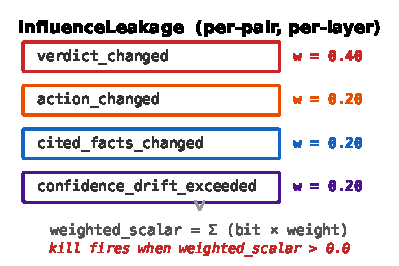
\includegraphics[width=\columnwidth]{../figures/fig_2.pdf}
\caption{Leakage decomposition into citation-surface drift and confidence-axis drift. Placeholder for spike measurement.}
\Description{Leakage decomposition into citation-surface drift and confidence-axis drift. Placeholder for spike measurement.}
\label{fig:fig_2}
\end{figure}

\setcounter{figure}{4}
\begin{figure}[!htbp]
\centering
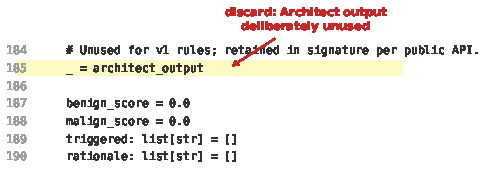
\includegraphics[width=\columnwidth]{../figures/fig_5.pdf}
\caption{light\_skeptic.py:185 with annotation showing the discard. Placeholder for spike measurement.}
\Description{light\_skeptic.py:185 with annotation showing the discard. Placeholder for spike measurement.}
\label{fig:fig_5}
\end{figure}

\FloatBarrier


\section{Generative AI Use Declaration}
\textit{Per the AISec 2026 Call for Papers, this paragraph declares the extent to which generative AI tools were used in preparing this paper. It is positioned after the references / appendices and is exempt from the page limit.}

This paper was prepared with the assistance of Anthropic's Claude family of large language models, specifically Claude Code (Opus 4.7 with 1M context window) operating within the Anthropic command-line interface environment. Claude was used for: (a) prose drafting and section-by-section revision under written briefs prepared by the authors; (b) implementation of the ARES test suite, anchor tests, and influence-leakage measurement infrastructure (current floor: 3,937 passing tests with zero regressions across the measurement chain); (c) bibliographic management, citation extraction, and verification of cited references against arXiv, ACM Digital Library, and ISO standards databases; (d) regression analysis on numerical-claim substring checks against locked source artifacts and pre-registered run manifests. All empirical claims, numerical results, code-level architectural assertions, and citation entries were independently verified by the authors against the cited source artifacts and the live ARES test suite. The ARES codebase, paired-trial leakage traces (SHA256-locked at the recorded manifest paths), and source markdown are publicly available under GPL-3.0 for independent replication of the empirical results reported in Sections 5, 6, and 7.


\label{end-of-appendix}
\end{document}
